\section{Register description}
\regover{
{\hyperref[gpip-gpadc-config]{gpadc\_config}}&GPADC configuration
\\
\hline
{\hyperref[gpip-gpadc-dma-rdata]{gpadc\_dma\_rdata}}&GPADC DMA read data
\\
\hline
{\hyperref[gpip-gpdac-config]{gpdac\_config}}&GPDAC configuration
\\
\hline
{\hyperref[gpip-gpdac-dma-config]{gpdac\_dma\_config}}&GPDAC dma configuration
\\
\hline
{\hyperref[gpip-gpdac-dma-wdata]{gpdac\_dma\_wdata}}&GPDAC dma write data
\\
\hline
{\hyperref[AON-gpadc-reg-cmd]{gpadc\_reg\_cmd}}&GPADC register configuration 0
\\
\hline
{\hyperref[AON-gpadc-reg-config1]{gpadc\_reg\_config1}}&GPADC register configuration 1
\\
\hline
{\hyperref[AON-gpadc-reg-config2]{gpadc\_reg\_config2}}&GPADC register configuration 2
\\
\hline
{\hyperref[AON-gpadc-reg-scn-pos1]{gpadc\_reg\_scn\_pos1}}&adc converation sequence 1
\\
\hline
{\hyperref[AON-gpadc-reg-scn-pos2]{gpadc\_reg\_scn\_pos2}}&adc converation sequence 2
\\
\hline
{\hyperref[AON-gpadc-reg-scn-neg1]{gpadc\_reg\_scn\_neg1}}&adc converation sequence 3
\\
\hline
{\hyperref[AON-gpadc-reg-scn-neg2]{gpadc\_reg\_scn\_neg2}}&adc converation sequence 4
\\
\hline
{\hyperref[AON-gpadc-reg-status]{gpadc\_reg\_status}}&GPADC register status
\\
\hline
{\hyperref[AON-gpadc-reg-isr]{gpadc\_reg\_isr}}&GPADC register operation
\\
\hline
{\hyperref[AON-gpadc-reg-raw-result]{gpadc\_reg\_raw\_result}}&GPADC register raw result
\\
\hline
{\hyperref[AON-gpadc-reg-define]{gpadc\_reg\_define}}&GPADC register define
\\
\hline
}

\subsection{gpadc\_config}
\label{gpip-gpadc-config}
Address:0x40002000
 \begin{figure}[H]
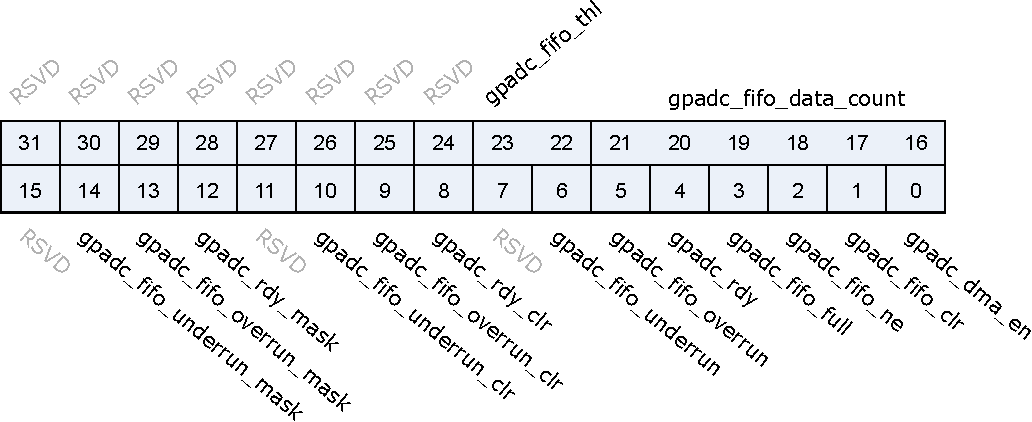
\includegraphics{gpip_gpadc_config.pdf}
\end{figure}

\regdes{31:24&RSVD& & & \\\hline
23:22&gpadc\_fifo\_thl&r/w&2'd0&fifo threshold \par 2'b00: 1 data  \par 2'b01: 4 data  \par 2'b10: 8 data \par 2'b11: 16 data
\\\hline
21:16&gpadc\_fifo\_data\_count&r&6'd0&fifo data number\\\hline
15&gpadc\_fifo\_rdy\_mask&r/w&1'b1&write 1 mask\\\hline
14&gpadc\_fifo\_underrun\_mask&r/w&1'b0&write 1 mask\\\hline
13&gpadc\_fifo\_overrun\_mask&r/w&1'b0&write 1 mask\\\hline
12&gpadc\_rdy\_mask&r/w&1'b0&write 1 mask\\\hline
11&RSVD& & & \\\hline
10&gpadc\_fifo\_underrun\_clr&w1c&1'b0&Write 1 to clear flag\\\hline
9&gpadc\_fifo\_overrun\_clr&w1c&1'b0&Write 1 to clear flag\\\hline
8&gpadc\_rdy\_clr&w1c&1'b0&Write 1 to clear flag\\\hline
7&gpadc\_fifo\_rdy&r&1'b0&FIFO ready interrupt flag\\\hline
6&gpadc\_fifo\_underrun&r&1'b0&FIFO underrun interrupt flag\\\hline
5&gpadc\_fifo\_overrun&r&1'b0&FIFO overrun interrupt flag\\\hline
4&gpadc\_rdy&r&1'b0&Conversion data ready interrupt flag\\\hline
3&gpadc\_fifo\_full&r&1'b0&FIFO full flag\\\hline
2&gpadc\_fifo\_ne&r&1'b0&FIFO not empty flag\\\hline
1&gpadc\_fifo\_clr&w1c&1'b0&FIFO clear signal\\\hline
0&gpadc\_dma\_en&r/w&1'b0&GPADC DMA enbale\\\hline

}
\subsection{gpadc\_dma\_rdata}
\label{gpip-gpadc-dma-rdata}
Address:0x40002004
 \begin{figure}[H]
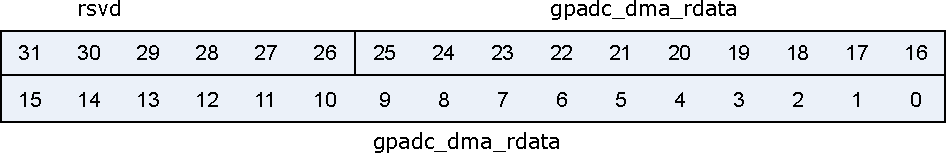
\includegraphics{gpip_gpadc_dma_rdata.pdf}
\end{figure}

\regdes{31:26&RSVD& & & \\\hline
25:0&gpadc\_dma\_rdata&r&26'd0&GPADC finial conversion result stored in the FIFO\\\hline

}
\subsection{gpdac\_config}
\label{gpip-gpdac-config}
Address:0x40002040
 \begin{figure}[H]
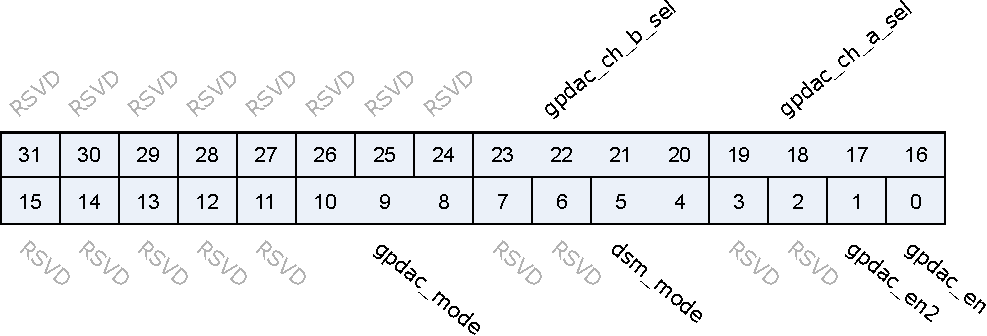
\includegraphics{gpip_gpdac_config.pdf}
\end{figure}

\regdes{31:24&RSVD& & & \\\hline
23:20&gpdac\_ch\_b\_sel&r/w&0&Channel B Source Select \par 0: Reg \par 1: DMA \par 2: DMA + Filter \par 3: Sin Gen \par 4: A (The same as channel A) \par 5: ~A (Inverse of channel A)
\\\hline
19:16&gpdac\_ch\_a\_sel&r/w&0&Channel A Source Select \par 0: Reg \par 1: DMA \par 2: DMA + Filter \par 3: Sin Gen
\\\hline
15:11&RSVD& & & \\\hline
10:8&gpdac\_mode&r/w&0&0:32k, 1:16k, 3:8k,  4:512k(for DMA only)\\\hline
7:6&RSVD& & & \\\hline
5:4&dsm\_mode&r/w&0&0:bypass, 1:dsm order=1, 2: dsm order=2\\\hline
3:2&RSVD& & & \\\hline
1&gpdac\_en2&r/w&0&GPDAC enable 2 (for B channel)\\\hline
0&gpdac\_en&r/w&0&GPDAC enable\\\hline

}
\subsection{gpdac\_dma\_config}
\label{gpip-gpdac-dma-config}
Address:0x40002044
 \begin{figure}[H]
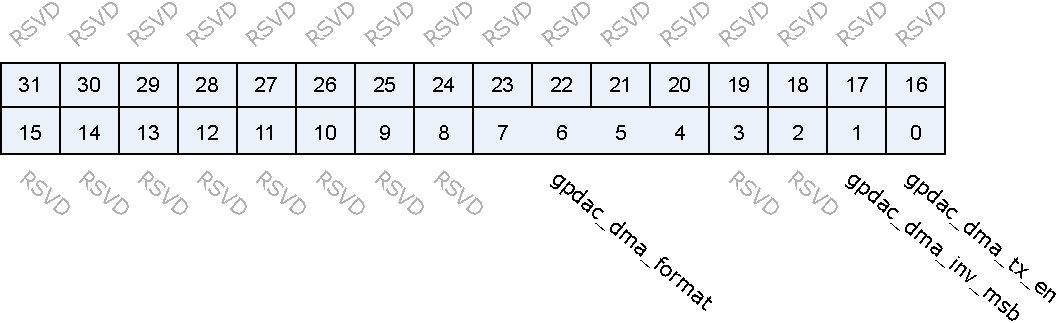
\includegraphics{gpip_gpdac_dma_config.pdf}
\end{figure}

\regdes{31:6&RSVD& & & \\\hline
5:4&gpdac\_dma\_format&r/w&0&DMA TX format (Data 12-bit) \par 0: {A0}, {A1}, {A2}… \par 1: {B0,A0}, {B1,A1}, {B2,A2}… \par 2: {A1,A0}, {A3,A2}, {A5,A4}… \par (Note: {20'h0,[11:0]} or {4'h0,[27:16],4'h0,[11:0]})
\\\hline
3:1&RSVD& & & \\\hline
0&gpdac\_dma\_tx\_en&r/w&0&GPDAC DMA TX enable\\\hline

}
\subsection{gpdac\_dma\_wdata}
\label{gpip-gpdac-dma-wdata}
Address:0x40002048
 \begin{figure}[H]
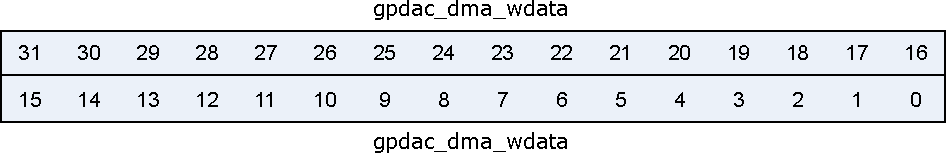
\includegraphics{gpip_gpdac_dma_wdata.pdf}
\end{figure}

\regdes{31:0&gpdac\_dma\_wdata&w&x&GPDAC DMA TX data\\\hline

}
\subsection{gpadc\_reg\_cmd}
\label{AON-gpadc-reg-cmd}
Address:0x4000f90c
\begin{figure}[H]
	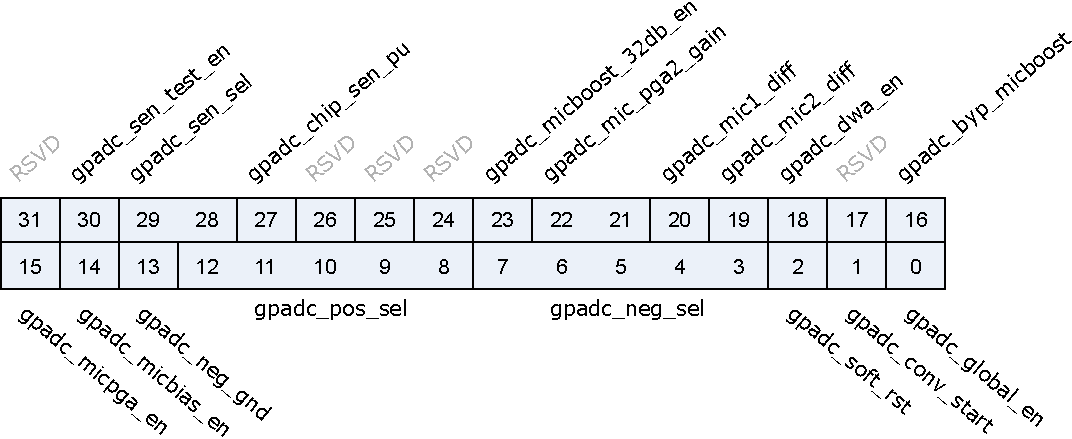
\includegraphics{AON_gpadc_reg_cmd.pdf}
\end{figure}

\regdes{31&RSVD& & & \\\hline
	30&gpadc\_sen\_test\_en&r/w&1'b0&enable sensor dc test mux \\\hline
	29:28&gpadc\_sen\_sel&r/w&2'h0&selected output current channel and measurement channel \par 2'h0: 1st channel \par 2'h1: 2nd channel \par 2'h2: 3rd channel  \par 2'h3: 4th channel
	\\\hline
	27&gpadc\_chip\_sen\_pu&r/w&1'b0&enable chip sensor test \par 1'b0: disable \par 1'b1: enable
	\\\hline
	26:24&RSVD& & & \\\hline
	23&gpadc\_micboost\_32db\_en&r/w&1'b0&micboost 32db enable \par 1'b0: 16dB \par 1'b1: 32dB
	\\\hline
	22:21&gpadc\_mic\_pga2\_gain&r/w&2'h0&mic\_pga2\_gain \par 2'h0: 0dB \par 2'h1: 6dB \par 2'h2: -6dB \par 2'h3: 12dB
	\\\hline
	20&gpadc\_mic1\_diff&r/w&1'b0&mic1 diff enable \par 1'b0: single \par 1'b1: diff
	\\\hline
	19&gpadc\_mic2\_diff&r/w&1'b0&mic2 diff enable \par 1'b0: single \par 1'b1: diff
	\\\hline
	18&gpadc\_dwa\_en&r/w&1'b0&dwa enable \par 1'b0: dwa disable \par 1'b1: dwa enable
	\\\hline
	17&RSVD& & & \\\hline
	16&gpadc\_byp\_micboost&r/w&1'b0&micboost amp bypass \par 1'b0: not bypass \par 1'b1: bypass
	\\\hline
	15&gpadc\_micpga\_en&r/w&1'b0&micpga enable \par 1'b0: micpga disable \par 1'b1: miapga enable
	\\\hline
	14&gpadc\_micbias\_en&r/w&1'b0&enable micbias  \par 1'b0: micbias power down \par 1'b1: miabias power on
	\\\hline
	13&gpadc\_neg\_gnd&r/w&1'b0&set negative input of adc to ground \par 1'b0: disable \par 1'b1: enable
	\\\hline
	12:8&gpadc\_pos\_sel&r/w&5'hf&select adc positive input in none-scan mode \par 5‘h0 gpio0 \par 5'h1 gpio1 \par 5'h2 gpio2 \par 5‘h3 gpio3 \par 5'h4 gpio4 \par 5'h5 gpio5 \par 5‘h6 gpio6 \par 5'h7 gpio7 \par 5'h8 gpio8 \par 5‘h9 gpio9 \par 5'h10 gpio10 \par 5'h11 gpio11 \par 5‘h12 daca \par 5'h13 dacb \par 5'h14 temp\_p \par 5‘h15 temp\_n \par 5'h16 vref \par 5'h17 atest \par 5‘h18 vbat/2 \par 5'h19 vp3\_diode \par 5'h20 vp2\_diode \par 5‘h21 vp1\_diode \par 5'h22 vp0\_diode \par 5'h23~31 avss
	\\\hline
	7:3&gpadc\_neg\_sel&r/w&5'hf&select adc positive input in none-scan mode \par 5‘h0 gpio0 \par 5'h1 gpio1 \par 5'h2 gpio2 \par 5‘h3 gpio3 \par 5'h4 gpio4 \par 5'h5 gpio5 \par 5‘h6 gpio6 \par 5'h7 gpio7 \par 5'h8 gpio8 \par 5‘h9 gpio9 \par 5'h10 gpio10 \par 5'h11 gpio11 \par 5‘h12 daca \par 5'h13 dacb \par 5'h14 temp\_p \par 5‘h15 temp\_n \par 5'h16 vref \par 5'h17 atest \par 5‘h18 vbat/2 \par 5'h19 vn3\_diode \par 5'h20 vn2\_diode \par 5‘h21 vn1\_diode \par 5'h22 vn0\_diode \par 5'h23~31 avss
	\\\hline
	2&gpadc\_soft\_rst&r/w&1'b0&user reset the whole block 1'h0: not reset  1'h1: reset  \\\hline
	1&gpadc\_conv\_start&r/w&1'b0&1'h0: stop converation  1'h1: start converation \\\hline
	0&gpadc\_global\_en&r/w&1'b0&1'h0: disable ADC  1'h1: enable ADC\\\hline
	
}
\subsection{gpadc\_reg\_config1}
\label{AON-gpadc-reg-config1}
Address:0x4000f910
\begin{figure}[H]
	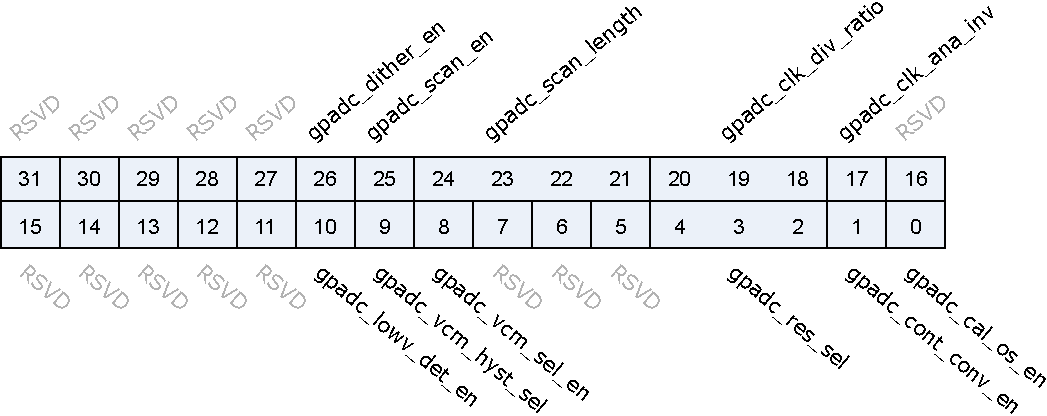
\includegraphics{AON_gpadc_reg_config1.pdf}
\end{figure}

\regdes{31&RSVD& & & \\\hline
	30:29&gpadc\_v18\_sel&r/w&2'h0&internal vdd18 select\\\hline
	28:27&gpadc\_v11\_sel&r/w&2'h0&internal vdd11 select\\\hline
	26&gpadc\_dither\_en&r/w&1'h0&Dither compensation enable\\\hline
	25&gpadc\_scan\_en&r/w&1'h0&select scan mode enable: 0: select  gpadc\_pos/neg\_sel;1: select  : select gpadc\_scan\_pos\_x and gpadc\_scan\_neg\_x\\\hline
	24:21&gpadc\_scan\_length&r/w&4'h0&select scan mode length \par 4'b0000 : select gpadc\_scan\_pos\_0 and gpadc\_scan\_neg\_0 \par 4'b0001 : select gpadc\_scan\_pos\_1 and gpadc\_scan\_neg\_1 \par 4'b0010 : select gpadc\_scan\_pos\_2 and gpadc\_scan\_neg\_2 \par 4'b0011 : select gpadc\_scan\_pos\_3 and gpadc\_scan\_neg\_3 \par 4'b0100 : select gpadc\_scan\_pos\_4 and gpadc\_scan\_neg\_4 \par 4'b0101 : select gpadc\_scan\_pos\_5 and gpadc\_scan\_neg\_5 \par 4'b0110 : select gpadc\_scan\_pos\_6 and gpadc\_scan\_neg\_6 \par 4'b0111 : select gpadc\_scan\_pos\_7 and gpadc\_scan\_neg\_7 \par 4'b1000 : select gpadc\_scan\_pos\_8 and gpadc\_scan\_neg\_8 \par 4'b1001 : select gpadc\_scan\_pos\_9 and gpadc\_scan\_neg\_9 \par 4'b1010 : select gpadc\_scan\_pos\_10 and gpadc\_scan\_neg\_10 \par 4'b1011 : select gpadc\_scan\_pos\_11 and gpadc\_scan\_neg\_11
	\\\hline
	20:18&gpadc\_clk\_div\_ratio&r/w&3'h3&analog 32M clock division ratio \par 3'b000: div=1 \par 3'b001: div=4 \par 3'b010: div=8 \par 3'b011: div=12 \par 3'b100: div=16 \par 3'b101: div=20 \par 3'b110: div=24 \par 3'b111: div=32
	\\\hline
	17&gpadc\_clk\_ana\_inv&r/w&1'b0&analog clock 2M inverted\\\hline
	16:11&RSVD& & & \\\hline
	10&gpadc\_lowv\_det\_en&r/w&1'b0&Low power supply detected enable\\\hline
	9&gpadc\_vcm\_hyst\_sel&r/w&1'b0&pga vcm hystersis select when vcm\_sel\_en is enabled\\\hline
	8&gpadc\_vcm\_sel\_en&r/w&1'b0&pga vcm selected when lowv\_det\_en is enable\\\hline
	7:5&RSVD& & & \\\hline
	4:2&gpadc\_res\_sel&r/w&3'h0&adc resolution/over-sample rate select  \par 3'b000    12bit 2MS/s, OSR=1  \par 3'b001    14bit 125kS/s, OSR=16 \par 3'b010    14bit 31.25kS/s, OSR=64  \par 3'b011    16bit 15.625KS/s, OSR=128 (voice mode16KS/s) \par 3'b100    16bit 7.8125KS/s, OSR=256 (voice mode 8KS/s)
	\\\hline
	1&gpadc\_cont\_conv\_en&r/w&1'b1&To enable continuous conversion \par 1'h0: one shot conversion  1'h1: continuous conversion
	\\\hline
	0&gpadc\_cal\_os\_en&r/w&1'b0&offset calibration enable\\\hline
	
}
\subsection{gpadc\_reg\_config2}
\label{AON-gpadc-reg-config2}
Address:0x4000f914
\begin{figure}[H]
	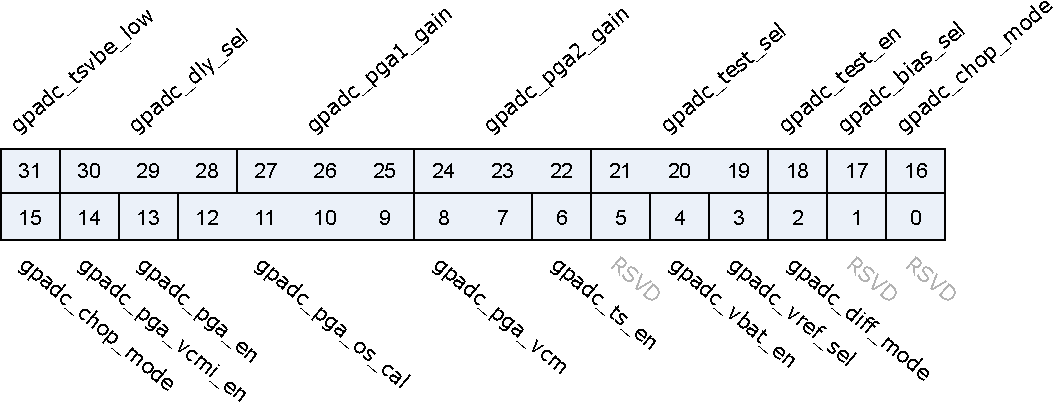
\includegraphics{AON_gpadc_reg_config2.pdf}
\end{figure}

\regdes{31&gpadc\_tsvbe\_low&r/w&1'b0&tsen diode current\\\hline
	30:28&gpadc\_dly\_sel&r/w&3'h0&adc conversion speed\\\hline
	27:25&gpadc\_pga1\_gain&r/w&3'h0&3'h0: disable \par 3'h1: gain=1 \par 3'h2: gain=2 \par 3'h3: gain=4 \par 3'h4: gain=8 \par 3'h5: gain=16 \par 3'h6: gain=32 \par 3'h7: gain=32
	\\\hline
	24:22&gpadc\_pga2\_gain&r/w&3'h0&3'h0: disable \par 3'h1: gain=1 \par 3'h2: gain=2 \par 3'h3: gain=4 \par 3'h4: gain=8 \par 3'h5: gain=16 \par 3'h6: gain=32 \par 3'h7: gain=32
	\\\hline
	21:19&gpadc\_test\_sel&r/w&3'h0&select test point 0~7\\\hline
	18&gpadc\_test\_en&r/w&1'b0&Analog test enable.\\\hline
	17&gpadc\_bias\_sel&r/w&1'b0&adc analog portion low power mode select \par 1'h0: bandgap system \par 1'h1:aon bandgap
	\\\hline
	16:15&gpadc\_chop\_mode&r/w&2'h3&2'b11    all  off \par 2'b11    Vref AZ on \par 2'b11    Vref AZ and PGA chop on \par 2'b11    Vref AZ and PGA chop+RPC on
	\\\hline
	14&gpadc\_pga\_vcmi\_en&r/w&1'b0&enable pga input vcm bias \\\hline
	13&gpadc\_pga\_en&r/w&1'b0&1'h0: disable PGA 1'h1 enable PGA\\\hline
	12:9&gpadc\_pga\_os\_cal&r/w&4'h8&pga offset calibration\\\hline
	8:7&gpadc\_pga\_vcm&r/w&2'h2&Audio PGA output common mode control \par 2'b00: cm=1.3V  \par 2'b11: cm=1.4V  \par 2'b11: cm=1.5V  \par 2'b11: cm=1.6V 
	\\\hline
	6&gpadc\_ts\_en&r/w&1'b0&1'h0: disable temperature sensor 1'h1: enable temperature sensor \\\hline
	5&gpadc\_tsext\_sel&r/w&1'b0&1'h0: internal diode mode  1'h1: external diode mode\\\hline
	4&gpadc\_vbat\_en&r/w&1'b0&1'h0: disable VBAT sensor 1'h1 enable VBAT sensor\\\hline
	3&gpadc\_vref\_sel&r/w&1'b0&ADC reference select  \par 1'h0 3.2V \par 1'h1 2.0V
	\\\hline
	2&gpadc\_diff\_mode&r/w&1'b0&1'h0 single-ended 1'h1 differential\\\hline
	1:0&RSVD& & & \\\hline
	
}
\subsection{gpadc\_reg\_scn\_pos1}
\label{AON-gpadc-reg-scn-pos1}
Address:0x4000f918
\begin{figure}[H]
	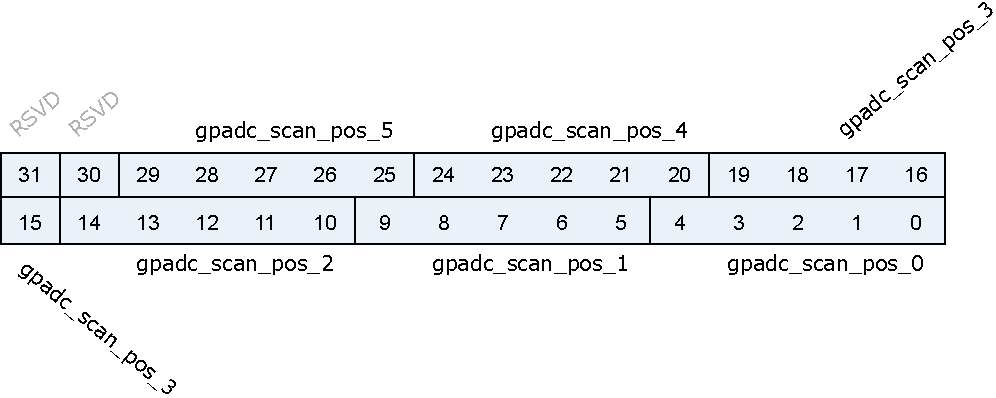
\includegraphics{AON_gpadc_reg_scn_pos1.pdf}
\end{figure}

\regdes{31:30&RSVD& & & \\\hline
	29:25&gpadc\_scan\_pos\_5&r/w&5'hf&definition is the same as adc\_reg\_cmd.adc\_pos\_sel\\\hline
	24:20&gpadc\_scan\_pos\_4&r/w&5'hf&definition is the same as adc\_reg\_cmd.adc\_pos\_sel\\\hline
	19:15&gpadc\_scan\_pos\_3&r/w&5'hf&definition is the same as adc\_reg\_cmd.adc\_pos\_sel\\\hline
	14:10&gpadc\_scan\_pos\_2&r/w&5'hf&definition is the same as adc\_reg\_cmd.adc\_pos\_sel\\\hline
	9:5&gpadc\_scan\_pos\_1&r/w&5'hf&definition is the same as adc\_reg\_cmd.adc\_pos\_sel\\\hline
	4:0&gpadc\_scan\_pos\_0&r/w&5'hf&definition is the same as adc\_reg\_cmd.adc\_pos\_sel\\\hline
	
}
\subsection{gpadc\_reg\_scn\_pos2}
\label{AON-gpadc-reg-scn-pos2}
Address:0x4000f91c
\begin{figure}[H]
	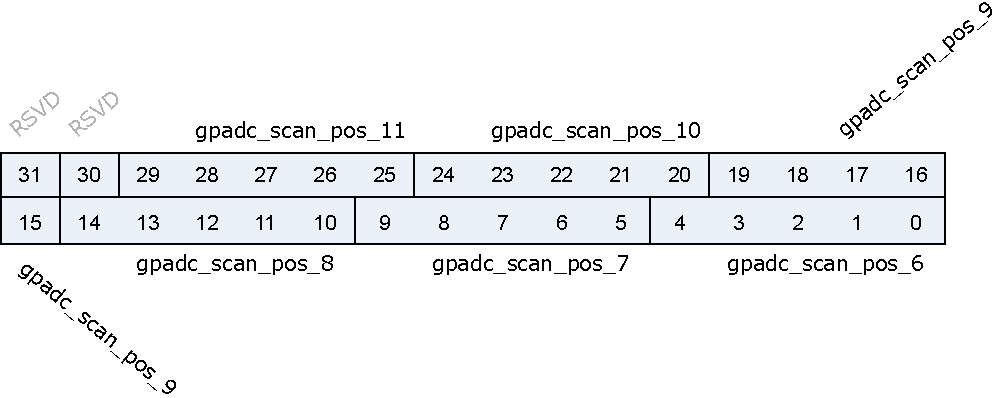
\includegraphics{AON_gpadc_reg_scn_pos2.pdf}
\end{figure}

\regdes{31:30&RSVD& & & \\\hline
	29:25&gpadc\_scan\_pos\_11&r/w&5'hf&definition is the same as adc\_reg\_cmd.adc\_pos\_sel\\\hline
	24:20&gpadc\_scan\_pos\_10&r/w&5'hf&definition is the same as adc\_reg\_cmd.adc\_pos\_sel\\\hline
	19:15&gpadc\_scan\_pos\_9&r/w&5'hf&definition is the same as adc\_reg\_cmd.adc\_pos\_sel\\\hline
	14:10&gpadc\_scan\_pos\_8&r/w&5'hf&definition is the same as adc\_reg\_cmd.adc\_pos\_sel\\\hline
	9:5&gpadc\_scan\_pos\_7&r/w&5'hf&definition is the same as adc\_reg\_cmd.adc\_pos\_sel\\\hline
	4:0&gpadc\_scan\_pos\_6&r/w&5'hf&definition is the same as adc\_reg\_cmd.adc\_pos\_sel\\\hline
	
}
\subsection{gpadc\_reg\_scn\_neg1}
\label{AON-gpadc-reg-scn-neg1}
Address:0x4000f920
\begin{figure}[H]
	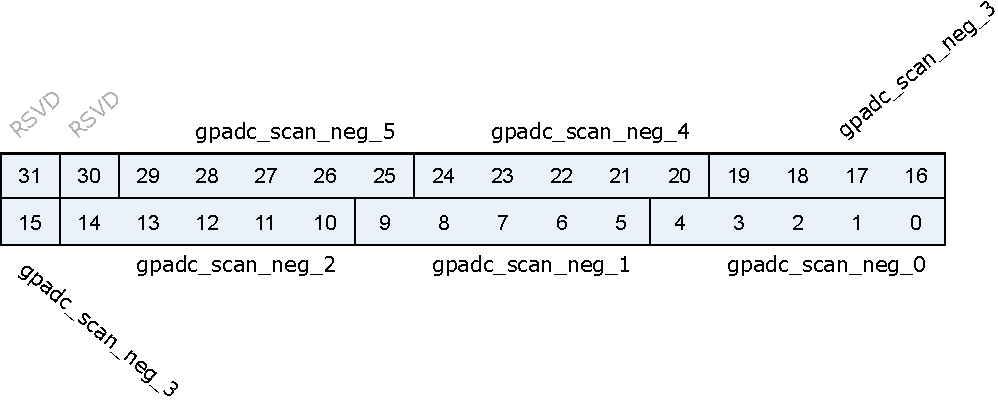
\includegraphics{AON_gpadc_reg_scn_neg1.pdf}
\end{figure}

\regdes{31:30&RSVD& & & \\\hline
	29:25&gpadc\_scan\_neg\_5&r/w&5'hf&definition is the same as adc\_reg\_cmd.adc\_neg\_sel\\\hline
	24:20&gpadc\_scan\_neg\_4&r/w&5'hf&definition is the same as adc\_reg\_cmd.adc\_neg\_sel\\\hline
	19:15&gpadc\_scan\_neg\_3&r/w&5'hf&definition is the same as adc\_reg\_cmd.adc\_neg\_sel\\\hline
	14:10&gpadc\_scan\_neg\_2&r/w&5'hf&definition is the same as adc\_reg\_cmd.adc\_neg\_sel\\\hline
	9:5&gpadc\_scan\_neg\_1&r/w&5'hf&definition is the same as adc\_reg\_cmd.adc\_neg\_sel\\\hline
	4:0&gpadc\_scan\_neg\_0&r/w&5'hf&definition is the same as adc\_reg\_cmd.adc\_neg\_sel\\\hline
	
}
\subsection{gpadc\_reg\_scn\_neg2}
\label{AON-gpadc-reg-scn-neg2}
Address:0x4000f924
\begin{figure}[H]
	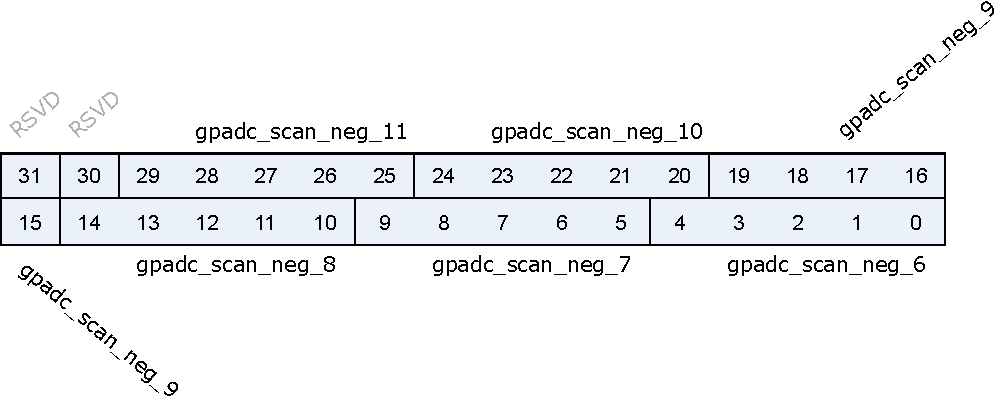
\includegraphics{AON_gpadc_reg_scn_neg2.pdf}
\end{figure}

\regdes{31:30&RSVD& & & \\\hline
	29:25&gpadc\_scan\_neg\_11&r/w&5'hf&definition is the same as adc\_reg\_cmd.adc\_neg\_sel\\\hline
	24:20&gpadc\_scan\_neg\_10&r/w&5'hf&definition is the same as adc\_reg\_cmd.adc\_neg\_sel\\\hline
	19:15&gpadc\_scan\_neg\_9&r/w&5'hf&definition is the same as adc\_reg\_cmd.adc\_neg\_sel\\\hline
	14:10&gpadc\_scan\_neg\_8&r/w&5'hf&definition is the same as adc\_reg\_cmd.adc\_neg\_sel\\\hline
	9:5&gpadc\_scan\_neg\_7&r/w&5'hf&definition is the same as adc\_reg\_cmd.adc\_neg\_sel\\\hline
	4:0&gpadc\_scan\_neg\_6&r/w&5'hf&definition is the same as adc\_reg\_cmd.adc\_neg\_sel\\\hline
	
}
\subsection{gpadc\_reg\_status}
\label{AON-gpadc-reg-status}
Address:0x4000f928
\begin{figure}[H]
	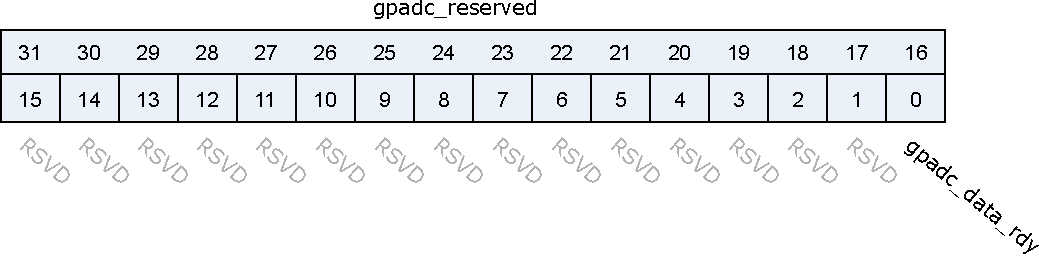
\includegraphics{AON_gpadc_reg_status.pdf}
\end{figure}

\regdes{31:16&gpadc\_reserved&r/w&16'h0&\\\hline
	15:1&RSVD& & & \\\hline
	0&gpadc\_data\_rdy&r&1'b0&ADC final conversion data ready\\\hline
	
}
\subsection{gpadc\_reg\_isr}
\label{AON-gpadc-reg-isr}
Address:0x4000f92c
\begin{figure}[H]
	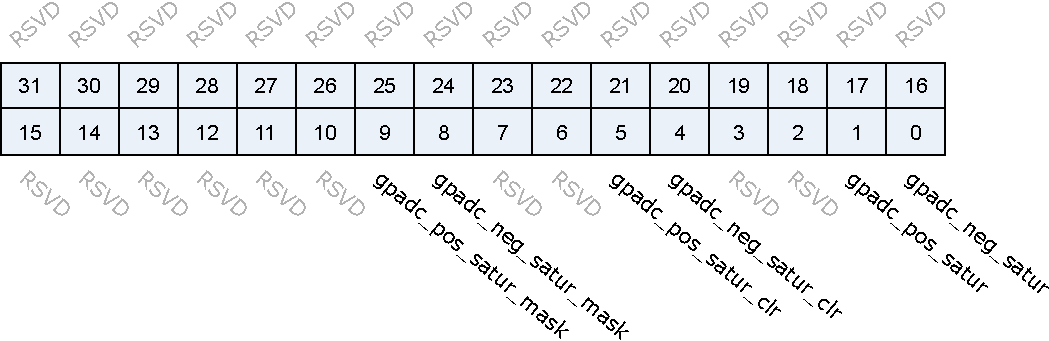
\includegraphics{AON_gpadc_reg_isr.pdf}
\end{figure}

\regdes{31:10&RSVD& & & \\\hline
	9&gpadc\_pos\_satur\_mask&r/w&1'h0&write 1 mask\\\hline
	8&gpadc\_neg\_satur\_mask&r/w&1'h0&write 1 mask\\\hline
	7:6&RSVD& & & \\\hline
	5&gpadc\_pos\_satur\_clr&r/w&1'b0&Write 1 to clear flag\\\hline
	4&gpadc\_neg\_satur\_clr&r/w&1'b0&Write 1 to clear flag\\\hline
	3:2&RSVD& & & \\\hline
	1&gpadc\_pos\_satur&r&1'b0&ADC data positive side saturation interrupt flag\\\hline
	0&gpadc\_neg\_satur&r&1'b0&ADC data negative side saturation interrupt flag\\\hline
	
}
\subsection{gpadc\_reg\_raw\_result}
\label{AON-gpadc-reg-raw-result}
Address:0x4000f934
\begin{figure}[H]
	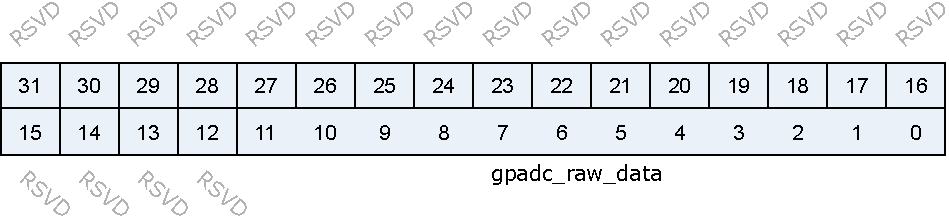
\includegraphics{AON_gpadc_reg_raw_result.pdf}
\end{figure}

\regdes{31:12&RSVD& & & \\\hline
	11:0&gpadc\_raw\_data&r&12'h0&ADC Raw data\\\hline
	
}
\subsection{gpadc\_reg\_define}
\label{AON-gpadc-reg-define}
Address:0x4000f938
\begin{figure}[H]
	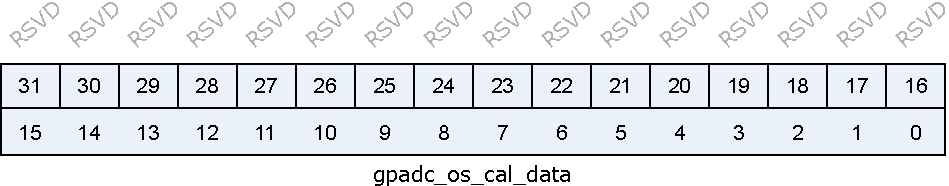
\includegraphics{AON_gpadc_reg_define.pdf}
\end{figure}

\regdes{31:16&RSVD& & & \\\hline
	15:0&gpadc\_os\_cal\_data&r/w&16'h0&User defined or self calculated offset data 16-bit signed \\\hline
	
}
